\chapter{PID控制器}

\section{PID控制器概述与其基本作用}

\subsection{比例控制器}

一个比例控制器的例子如下：
\begin{center}
    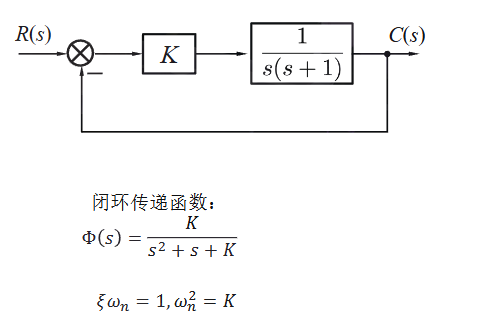
\includegraphics[width = .5\textwidth]{note/PID design/figure/1.png}
\end{center}

\textbf{比例控制器有以下的优点：}
\begin{enumerate}
    \item 提高系统稳态精度
    \item 提高系统的快速性
    \item 降低稳定裕度
\end{enumerate}

\subsection{PD控制器}

一个PD控制器的例子如下：
\begin{center}
    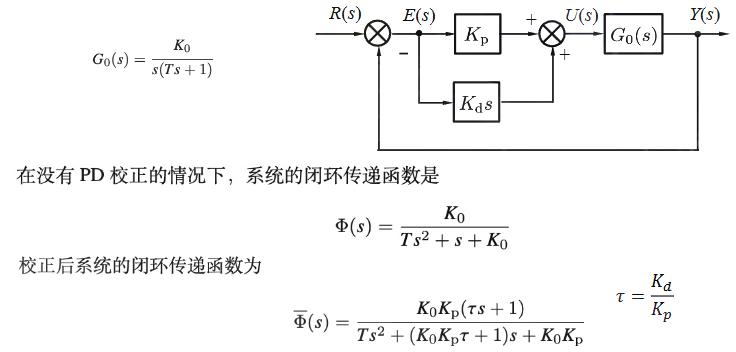
\includegraphics[width = .5\textwidth]{note/PID design/figure/2.png}
\end{center}

\textbf{PD控制器有以下优点：}
\begin{enumerate}
    \item 改变系统的自然震荡频率和阻尼比
    \item 提高系统的动态性能，加快响应速度，提高系统的稳定性
\end{enumerate}

\subsection{PI控制器}

PI控制器的一般形式如下：
\begin{center}
    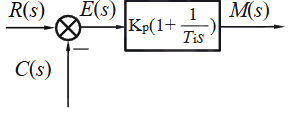
\includegraphics[width = .3\textwidth]{note/PID design/figure/3.png}
\end{center}

PI控制器相当于积分环节和一阶微分环节串联，几分环节改变系统型别，一阶微分环节系统的自然频率和阻尼比，保证闭环系统的稳定性，所以\textbf{PI控制器有以下的优点：}
\begin{enumerate}
    \item 提高系统的型别
    \item 提高系统的动态性能
\end{enumerate}

\textbf{
\begin{itemize}
    \item 对于单一的积分控制器，可以提高系统的型别，以消除或减弱稳态误差
    \item 如果系统不可变部分已有积分环节，再采用单一的积分控制可能导致系统不稳定，故此时可以引入PI控制器
    \item PI控制通过在原点增加极点来"消灭"稳态误差，但是代价是把根轨迹向右“挤”，如果积分作用太强($T_i$太小)，系统超调会猛增，甚至失控
\end{itemize}
}

\subsection{PID控制器}

PID控制器的一般形式如下：
\begin{center}
    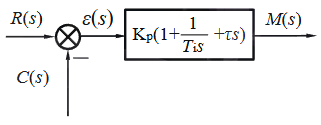
\includegraphics[width = .3\textwidth]{note/PID design/figure/4.png}
\end{center}

\textbf{PID控制器具有以下的优点：}
\begin{enumerate}
    \item 提高系统的型别
    \item 通过合适选择参数，还将为系统增加两个开环零点，在提高系统动态性能方面具有更大的优越性
\end{enumerate}

\section{PID参数整定}

\subsection{动态响应法}
以传递函数为$G(s) = \frac{K e^{-\tau s}}{Ts + 1}$为例来介绍这种方法，具体步骤如下：
\begin{enumerate}
    \item 求取动态阶跃响应曲线，求得如下：
    \begin{center}
        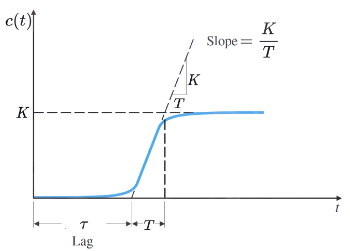
\includegraphics[width = .4\textwidth]{note/PID design/figure/5.png}
    \end{center}
    \item 估计被控对象的传递函数，将其拐点切线和时间轴和$c(t) = K$的交点可得到$\tau$和$T$的值，如上图所示
    \item 由Ziegler-Nichols给出的调整法则表，确定PID参数，具体如下：
    \begin{center}
        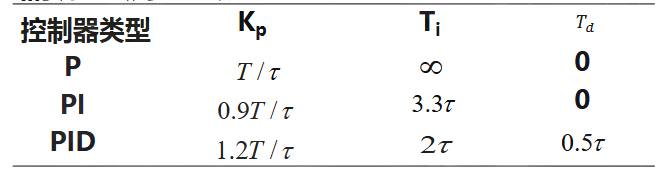
\includegraphics[width = .4\textwidth]{note/PID design/figure/6.png}
    \end{center}
    \item 由上表可以确定控制器的具体传递函数，根据选用P/PI/PID控制器而定
\end{enumerate}

使用动态响应法有几点注意事项：
\begin{enumerate}
    \item 系统开环下测出阶跃响应
    \item 闭环单位阶跃响应为S形
    \item 这种方法能保证阶跃响应的暂态分量最大峰值和第二峰值之比为4:1，$\xi \approx 0.21$
    \item \textbf{被控对象有几分环节和复数极点时不适用}
\end{enumerate}

\subsection{临界增益法}

\textbf{临界增益法在系统闭环情况下进行}，示意图如下：
\begin{center}
    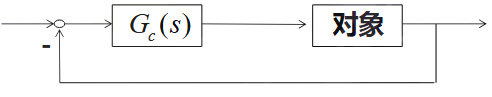
\includegraphics[width = .5\textwidth]{note/PID design/figure/7.png}
\end{center}

具体步骤如下：
\begin{enumerate}
    \item 令$I_i = \infty , T_d = 0$，将控制器设置为比例控制，将$K_p$从0增大，首次出现等幅振荡时，记下此时的增益$K_{ps}$和振荡周期$T_s$
    \item 根据Ziegler-Nichols给出的调整法则表，确定PID参数，具体如下：
    \begin{center}
        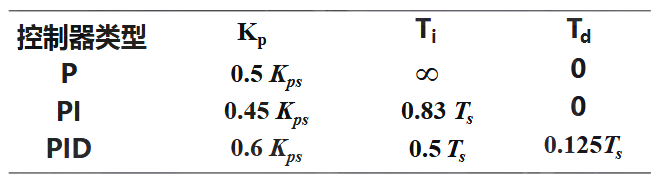
\includegraphics[width = .3\textwidth]{note/PID design/figure/8.png}
    \end{center}
\end{enumerate}

\textbf{以上两种方法均用到了Z-N法给出的参数，但是这个参数往往会让超调$>60\%$，在实际工程中，我们需要手动微调PID零点位置，来压低超调量}

\section{离散PID}

\begin{center}
    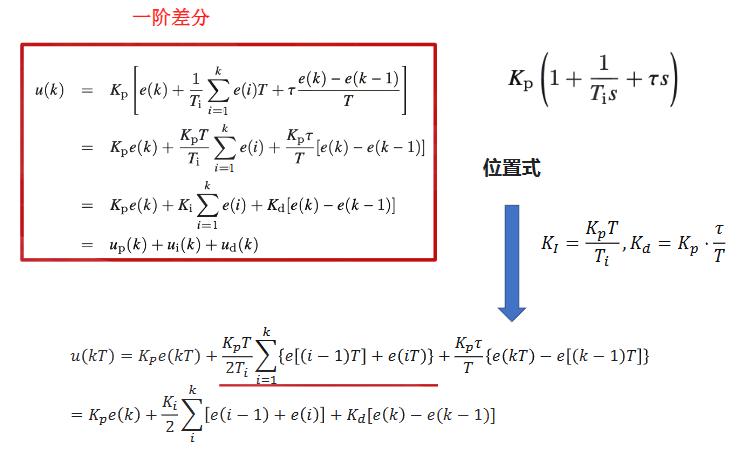
\includegraphics[width = .6\textwidth]{note/PID design/figure/9.png} \\
    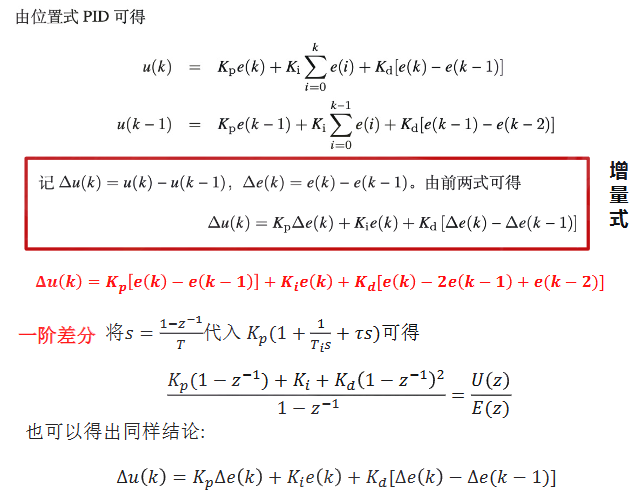
\includegraphics[width = .6\textwidth]{note/PID design/figure/10.png} \\
    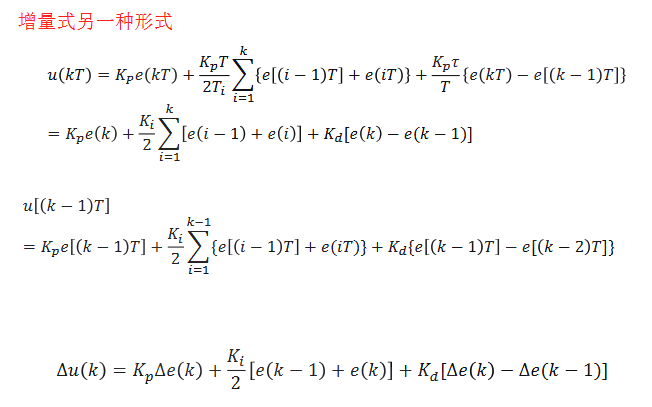
\includegraphics[width = .6\textwidth]{note/PID design/figure/11.png}
\end{center}
